%\pdfminorversion=6
\documentclass[10pt]{amsart}
\usepackage[margin=1.2in]{geometry}
% \usepackage{geometry}
\usepackage[export]{adjustbox}
% \setlength{\oddsidemargin}{.25in}
% \setlength{\evensidemargin}{.25in} 
% \setlength{\topmargin}{.25in}
% \setlength{\headsep}{.25in}
% \setlength{\headheight}{0in}
% \setlength{\textheight}{8.5in}
% \setlength{\textwidth}{6in} 
% \usepackage{quiver}



%%%%%%%%%%%%%%%%%%%%%%%%%%
%%%%%%% PACKAGES %%%%%%%%%
%%%%%%%%%%%%%%%%%%%%%%%%%%
\usepackage{amsmath, amsthm, amssymb} % standard stuff
\usepackage{pdflscape}
\usepackage{fourier}


\usepackage[dvipsnames]{xcolor}
\usepackage[colorlinks, allcolors=OliveGreen]{hyperref} 
\hypersetup{
    colorlinks = true,
    linkcolor = OliveGreen,
    citecolor = Blue,
    urlcolor = Blue,
}
\usepackage{tikz-cd} 
\usepackage{tikz}
\usepackage[nameinlink,capitalize]{cleveref} 
\usepackage{mathtools}
\usepackage[shortlabels]{enumitem} 
\usepackage{microtype} 
\usepackage{mathrsfs}
\usepackage{lscape}
\usepackage{float}
\usepackage{multicol}
\usepackage{euscript}
\newcommand{\euscr}[1]{\EuScript{#1}}
\newtheorem{thm}{Theorem}[section]
\newtheorem{conj}[thm]{Conjecture}
\newtheorem{proposition}[thm]{Proposition}
\newtheorem{corollary}[thm]{Corollary}
\newtheorem{lemma}[thm]{Lemma}
\newtheorem{question}[thm]{Question}
\theoremstyle{definition}
\newtheorem{rmk}[thm]{Remark}
\newtheorem{ex}[thm]{Example}
\newtheorem{watchout}[thm]{\warning \textbf{Warning} \warning}
\newtheorem{exercise}[thm]{Exercise}
\usepackage[
    backend=biber,
    style=alphabetic,
    maxbibnames=99,
    isbn=false,
    url=false,
    doi=false,
    maxalphanames=9,
    minalphanames=4,
]{biblatex}
% \addbibresource{References.bib} 
\renewcommand*{\bibfont}{\small}
\newcommand{\cdef}[1]{\textcolor{Bittersweet}{#1}}
\DeclareFontFamily{T1}{cbgreek}{}
\DeclareFontShape{T1}{cbgreek}{m}{n}{<-6>  grmn0500 <6-7> grmn0600 <7-8> grmn0700 <8-9> grmn0800 <9-10> grmn0900 <10-12> grmn1000 <12-17> grmn1200 <17-> grmn1728}{}
\DeclareSymbolFont{quadratics}{T1}{cbgreek}{m}{n}
\DeclareMathSymbol{\quadf}{\mathord}{quadratics}{21}
\newcommand{\dq}{\euscr{DQ}}

\newcommand{\aeu}{\euscr{A}}
\newcommand{\cc}{\mathbb{C}}
\newcommand{\ff}{\mathbb{F}}
\newcommand{\mm}{\mathbb{M}}
\newcommand{\rr}{\mathbb{R}}
\renewcommand{\ss}{\mathbb{S}}
\newcommand{\zz}{\mathbb{Z}}


\newcommand{\upe}{\textup{E}}
\newcommand{\uph}{\textup{H}}
\newcommand{\hsf}{\textup{\textsf{h}}}
\newcommand{\upbo}{\textup{bo}}
\newcommand{\upkgl}{\textup{kgl}}
\newcommand{\upkq}{\textup{kq}}
\newcommand{\up}[1]{\textup{#1}}
\newcommand{\upx}{\textup{X}}

\renewcommand{\bar}[1]{\overline{#1}}
\newcommand{\sser}[4]{\prescript{#1}{#2}{\textup{E}}_{#3}^{#4}}
\newcommand{\invamalg}{\mathbin{\rotatebox[origin=c]{180}{$\amalg$}}}

\newcommand{\ycw}{\textup{Y}^{\mathbb{C}}_{(\eta, \nu)}}
\newcommand{\yw}{\textup{Y}_{(\eta, \nu)}}
\newcommand{\yv}{\textup{Y}_{(\hsf, \eta)}}
\newcommand{\ywtop}{\textup{Y}^\textup{top}_{(\eta, \nu)}}
\newcommand{\yvtop}{\textup{Y}^\textup{top}_{(2, \eta)}}


\setcounter{tocdepth}{2}

%%% MACROS
\newcommand\setItemnumber[1]{\setcounter{enumi}{\numexpr#1-1\relax}}

%%% TYPEFACES 
\newcommand{\ul}{\underline}
\newcommand{\mf}{\mathfrak}

%%% SPECIAL LETTERS
\newcommand{\A}{\mathbb{A}} % blackboard bold A
\newcommand{\fa}{\mathfrak{a}} % gothic font a
\newcommand{\fb}{\mathfrak{b}} % gothic font b
\newcommand{\uA}{\underline{\mathrm{A}}} % underlined A
\newcommand{\C}{\mathbb{C}} % blackboard bold C
\newcommand{\F}{\mathbb{F}} % blackboard bold F
\newcommand{\N}{\mathbb{N}} % blackboard bold N
\newcommand{\fp}{\mathfrak{p}} % gothic font p
\newcommand{\QQ}{\mathbb{Q}} % blackboard bold Q
\newcommand{\fq}{\mathfrak{q}} % gothic font q
\newcommand{\Q}{\mathtt{Q}} % Q as in the proposition
\newcommand{\R}{\mathbb{R}}
\newcommand{\Z}{\mathbb{Z}} % blackboard bold Z

%%% OPERATORS
\DeclareMathOperator{\Hom}{Hom} % Hom set
\DeclareMathOperator{\Fun}{Fun} % functors
\DeclareMathOperator{\Spec}{Spec} % prime ideal spectrum
\DeclareMathOperator{\id}{id} % identity
\DeclareMathOperator{\modmod}{/\!/}
\DeclareMathOperator{\ext}{\text{Ext}}
\newcommand{\colim}{\operatorname{colim}}
\newcommand{\shk}{\text{SH}(k)}
\newcommand{\spc}{\text{Spc}}

%BOLD SPECTRA%%%%%
\newcommand{\KGL}{\textbf{KGL}}
\newcommand{\kgl}{\textbf{kgl}}

\newcommand{\KO}{\textbf{KO}}
\newcommand{\ko}{\textbf{ko}}
\newcommand{\KU}{\textbf{KU}}
\newcommand{\ku}{\textbf{ku}}
\newcommand{\HZ}{\textbf{H}\mathbb{Z}}
\newcommand{\HF}{\textbf{H}\mathbb{F}}

%%%BP<n> STUFF%%%
\newcommand{\bpgl}[1]{\text{BPGL}\langle #1 \rangle}





%%% CATEGORIES
% Style guide: most pre-existing categories (CRing, Set, etc. in \mathsf)
% Except polynomial category (in \mathcal)
\newcommand{\CRing}{\mathsf{CRing}} % commutative 

% Shorter dash, for use in stuff like R-mod, G-set, etc.
% from https://tex.stackexchange.com/a/642931/15197
\DeclareMathSymbol{\mhyphen}{\mathord}{AMSa}{"39}

%%% THEOREMS
\numberwithin{equation}{section} % number the equations as 1.1, 1.2, ... instead of just 1, 2, ... 

\newtheorem{letterthm}{Theorem}
\renewcommand*{\theletterthm}{\Alph{letterthm}}
% \newtheorem{thm}[Theorem]{Theorem}
% \newtheorem{proposition}[Proposition]{Proposition}
% \newtheorem{lemma}[Lemma]{Lemma}
% \newtheorem{question}[Question]{Question}
% \newtheorem{goal}[Goal]{Goal}
% \newtheorem{corollary}[Corollary]{Corollary}
\newtheorem*{thm*}{Theorem}
\newtheorem*{corollary*}{Corollary}
\newtheorem*{lemma*}{Lemma}
\newtheorem*{proposition*}{Proposition}




\theoremstyle{definition}
\newtheorem{definition}[equation]{Definition}
\newtheorem{notation}[equation]{Notation}
\newtheorem{example}[equation]{Example}

%%%SS STUFF%%%
\newcommand{\E}[2]{\prescript{#1}{#2}{E}}



%%% EDITING MACROS
\usepackage[textwidth=25mm, textsize=tiny]{todonotes}
\usepackage[dvipsnames]{xcolor}
\usepackage{tcolorbox}
\usepackage{color}
\definecolor{orange'}{HTML}{D55E00}


%Jackson's Notes
\newcommand{\jmmar}[1]{\todo[color=orange'!50!white,linecolor=orange'!50!white,size=\tiny]{JM: #1}}
\newcommand{\jmil}[1]{\todo[inline,color=orange'!50!white,linecolor=orange'!50!white,size=\normalsize]{JM: #1}}

%%%%%%%%%%%%%%%%%%%%%%%
%%% DOCUMENT BEGINS %%%
%%%%%%%%%%%%%%%%%%%%%%%
\begin{document}

%%% TITLE %%%
\title{MATH 480: Homotopy Theory Final Project}
% \author{}
% \address{Department of Mathematics, University of Washington, Seattle, Washington}
% \email{\href{mailto:jackmann@uw.edu}{jackmann@uw.edu}}


% 14F42: motivic cohomology; motivic homotopy theory
% 55Q10: Stable homotopy groups,
% 55T15: Adams spectral sequences
% \subjclass[2020]{14F42, 55Q51, 55T15}

%%% ABSTRACT 
\begin{abstract}
    This is a draft of a topics list for the final project in this course. 
    This version is from \textbf{Wednesday, April 8}.
\end{abstract}

\maketitle
\tableofcontents

\section{Instructions}
As a final project for this course, you will write an expository paper on one of the topics listed  below (or, if you have an idea not listed, come talk to me). I will continually update this list of topics throughout the quarter. I have also tried to sort the projects by their flavor, either algebraic, topological, or categorical. This sorting is entirely subjective, and each project can certainly have elements of all flavors.


The guidelines for this project are simple:
\begin{itemize}
    \item At least 10 pages of mathematical writing.
    \item Typeset in LaTeX.
    \item A balance of mathematical content (lemmas, propositions, theorems, corollaries, and their proofs) along with tasteful discussion (why should we care about this topic, what is the big picture, where does this topic fit into the grand scheme of homotopy theory, etc).
\end{itemize}
\textbf{Before getting started,} be sure to come and okay your topic with me. I will schedule one-on-one meetings with everybody at least once over the course of the quarter. If you have any questions, feel free to reach out to me at any time.

\section{Topics}
Here are some potential topics for final projects. Remember, these are only suggestions, and this list is a work in progress! You are welcome to write about any topic you want, so long as you confirm it with me.

\subsection{More of a $\sim$topology$\sim$ flavor}
\subsection*{Configuration spaces}
Let $X$ be a topological space and let $X^n \coloneq X \times \cdots \times X$ $n$-times. The \cdef{\emph{ordered configuration space}} $\text{Conf}_n(X)$ is the set of all pairwise distinct collections of $n$ points in $X$:
\[
    \mathrm{Conf}_n(X) = \{(x_i) \in X^n : x_i \neq x_j \text{ for all }i\neq j\}.
\]
Note that this space has a natural permutation action by the symmetric group, denoted here as $\Sigma_n$. The \cdef{\emph{unordered configuration space}} $\text{UConf}_n(X)$ is the orbit space of this group action:
\[
    \text{UConf}_n(X) = \text{Conf}_n(X)/\Sigma_n.
\]
For example, for any two points $x_1, x_2 \in X$, the sequences $(x_1,x_2)$ and $(x_1, x_2)$ are distinct points in $\text{Conf}_2(X)$; however, there is a transposition $(1 \,2) \in \Sigma_2$ which acts by on our sequence by $(x_1, x_2) \mapsto (x_2, x_1)$, hence they are in the same orbit and thus represent the same point in $\text{UConf}_2(X)$.

Configuration spaces are very useful in homotopy theory in many ways. Here are a few of them.
\begin{itemize}
    \item The fundamental groups of the ordered and unordered configuration space on $n$ elements are the $n$-strand braid group and the pure $n$-strand braid group. Braid groups come up a lot in physics, TQFTs, representation theory, and knot theory.
    \item The configuration space $\text{Conf}_n(\mathbb{R}^2)$ and $\text{UConf}_n(\mathbb{R}^2)$ are examples of Eilenberg--MacLand spaces of type $\text{K}(\pi, 1)$.
    \item Configuration spaces are a type of moduli space.
\end{itemize}

\textbf{References:}
\begin{itemize}
    \item Here is a nice article: \href{https://arxiv.org/pdf/1911.11186}{https://arxiv.org/pdf/1911.11186}.
    \item \href{https://ncatlab.org/nlab/files/Cohen-IntroConfigSpaces.pdf}{Notes by Fred Cohen}.
\end{itemize}

\subsection*{Universal covers and covering spaces}
Something very useful in computing $\pi_1(S^1)$ was the existence of a continuous surjection $p:\mathbb{R} \to S^1$. The properties that were nice were that $\mathbb{R}$ was connected and locally path-connected and contractible, and that every point $x \in S^1$ had some open neighborhood $U$ such that the preimage $p^{-1}(U) \subseteq \mathbb{R}$ was a disjoint union of open sets in $\mathbb{R}$, each of which was homeomorphic to $U$.

The map $p:\mathbb{R} \to S^1$ along with these properties describes $p$ as a \cdef{\emph{covering map}}. More generally, we can talk about covers $q:E \to X$ of arbitrary topological spaces. these share all of the same properties as the map $p:\mathbb{R} \to S^1$ apart from the fact that we don't require $E$ to be contractible. Some really cool things come into the theory of covering spaces:
\begin{itemize}
    \item For any point $x \in X$ in the base space, the fundamental group $\pi_1(X, x)$ acts transitively on the fiber $q^{-1}(x)$. This action is known as the\cdef{\emph{monodromy action}}.
    \item If $X$ is simply connected, then $q$ is a homeomorphism.
    \item For $n \geq 2$, the induced map $q_*:\pi_1(E, q^{-1}(x)) \to \pi_1(X, x)$ is an isomorphism.
    \item Every connected and locally path-connected space admits a covering map from some simply connected space $\tilde{X}$. This is known as the \cdef{\emph{universal cover}}.
    \item If $X$ admits a universal over, then there is a one-to-one correspondence between conjugacy classes of subgroups of $\pi_1(X)$ and isomorphism classes of covers $E \to X$.
\end{itemize}

\textbf{References:}
\begin{itemize}
    \item Chapters 11 and 12 of ``Introduction to Topological Manifolds'' by Jack Lee.
    \item Section 1.3 of \href{https://pi.math.cornell.edu/~hatcher/AT/AT.pdf}{``Algebraic Topology"} by Allen Hatcher.
\end{itemize}

\subsection*{Cobordism of manifolds}
A \cdef{\emph{manifold}} of dimension $n$ is a topological space $M$ which is second-countable, Hausdorff, and such that for every point $p \in M$, there is an open neighborhood $U$ of $p$ which is homeomorphic to an open subset of $\mathbb{R}^n$. So, \emph{locally}, $M$ looks like Euclidean space, but it may have some interesting global structure. For example, the torus $\mathbb{T} = S^1 \times S^1$ is a 2-manifold, the sphere $S^n$ is an $n$-manifold, the Klein Bottle is a $2$-manifold. A \cdef{\emph{closed manifold}} is a manifold which is compact and without boundary. All of the examples I gave are closed manifolds.

Let $M, N$ be two closed $n$-manifolds. A \cdef{\emph{cobordism}} between $M$ and $N$ is an $n+1$-dimensional compact manifold $W$ with boundary such that:
\begin{itemize}
    \item there are embeddings $i:M \to \partial W$ and $j:N \to \partial W$;
    \item the boundary of $W$ consists of two disjoint copies of $M$ and $N$ and nothing else:
    \[
    \partial W = i(M) \amalg j(N).
    \]
\end{itemize}
Here is a picture of a cobordism.
\begin{figure}[H]
    \centering
    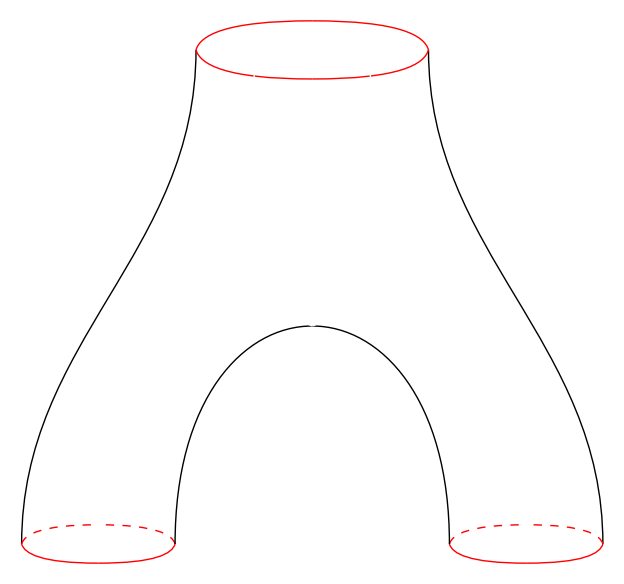
\includegraphics[scale=.35]{cob.png}
    \caption{The pair of pants manifold (which is a 2-manifold) is a cobordism between the top red circle $M = S^1$ (which is a 1-manifold) and the bottom red circles $N = S^1 \amalg S^1$ (which is a 1-manifold.}
    \label{fig:cobordism}
\end{figure}
In this way, you can kind of think of the $(n+1)$-manifold as parameterizing a way to continuously go from $M$ to $N$ in a way that is different than a homotopy. In the example we just gave, $M$ and $N$ are not homotopy equivalent, but the do have a cobordism between them. We say that $M$ and $N$ are \cdef{\emph{cobordant}}.

Cobordisms are really, really useful in homotopy theory.
\begin{itemize}
    \item One can ask for the manifolds $M$ and $N$ to have structure and for a cobordism $W$ between them to respect this structure. This leads to oriented cobordism, complex cobordism, framed cobordism, unoriented cobordism, and more and more.
    \item Cobordism defines an equivalence relation on the set of all $n$-dimensional manifolds. We denote the set of cobordism classes of $n$-manifolds by $\Omega_n$. In fact, $\Omega_n$ forms a group under connect sum. More interestingly, if we clue together all dimensions, the resulting graded abelian group
    \[\Omega_* = \bigoplus_{n \geq 0} \Omega_n\]
    is a ring! These rings are well studied, sometimes have an incredible interpretation, and sometimes have an unknown answer.
    \item Cobordism is very related to surgery theory.
    \item Cobordism is very related to TQFTs (in fact, are used in the definition of a TQFT!).
\end{itemize}

\textbf{References:}
\begin{itemize}
    \item \href{https://web.ma.utexas.edu/users/dafr/bordism.pdf}{Dan Freed's notes}
\end{itemize}

% \subsection{TQFTs}

\subsection*{Group actions on spaces}
In this course, we have studied the homotopy theory of topological spaces. However, there are many other objects whose ``homotopy theory" we may study. A particular example that occurs very frequently is the homotopy of \emph{\cdef{equivariant topological spaces}}, otherwise known as \emph{\cdef{equivariant homotopy theory}}. This is the homotopy theory of topological spaces equipped with the action of a group $G$. 

A group action of $G$ on a space $X$ is a map $G \times X \to X$ such that
\begin{itemize}
    \item $g_1 \cdot (g_2 \cdot x) = (g_1 g_2) \cdot x$ for any elements $g_1, g_2 \in G$, and
    \item $e \cdot x=x$ for every $x \in X$, where $e\in G$ is the identity element.
\end{itemize}
Notice that it doesn't make sens to ask for the action to be continuous unless we are requiring $G$ to be a topological group. 

Examples of group actions on spaces are not hard to come by. One should think of group actions as encoding some sort of symmetry of your space.
\begin{itemize}
    \item Any group $G$ acts trivially on any space $X$: just define the action to be $g \cdot x = x$ for any $g \in G$.
    \item The cyclic group of order two $C_2$ acts on any sphere $S^n$ by 
    \[\gamma \cdot x = -x,\]
    where $\gamma$ is the nontrivial element. This is the action which sends each point to its antipode.
    \item The symmetric group on $n$ elements $\Sigma_n$ acts by permutation on any set with $n$-elements. In this way, $\Sigma_n$ acts on Euclidean space $\mathbb{R}^n$ by permutating the standard basis. The one point compactification of $\mathbb{R}^n$ is the sphere $S^n$, and the action of $\Sigma_n$ lifts to an action on $S^n$. 
    \item More generally, let $V$ be any real vector space with an action of a group $G$. For example, we could take $V$ to be $\mathbb{R}^3$ with the action of the cyclic group $C_3$ given by $\gamma \cdot  (x, y, z) = (z, x, y)$ and $\gamma^2 \cdot (x, y, z) = (y,z,x)$. The one point compactification of $V$ is, as a \emph{nonequivariant} topological space, homoemorphic to a sphere $S^n$. However, the action of $G$ lifts to an action on $S^n$, which is far different than the trivial action on $S^n$ which always exists. Thus, to indicate that the one point compactification of $V$ is \emph{equivariantly} different from $S^n$, we denote this space by $S^V$. This is known as a \cdef{\emph{representation sphere}}, as $V$ is an example of a \cdef{\emph{representation}} of the group $G$.
\end{itemize}
If we are working with spaces with extra structure, such as equivariant spaces, we want morphisms which respect this structure. A map of $G$-spaces then is a continous map of spaces $f:X \to Y$ such that
\[
g \cdot f(x) = f(g \cdot x).
\]
In other words, the map commutes with the action.

Equivariant topology and equivariant homotopy theory have been hot topics in research for many years, and they are amenable to study from a variety of perspectives. For example, there is a slick interpretation of the category $\euscr{T}\mathrm{op}^G$ of $G$-equivariant spaces in the following way. There is a category $\mathcal{O}_G$ known as the \cdef{\emph{orbit category}}, whose objects are the cosets $G/H$ where $H$ is a subgroup of $G$ (not necessarily normal!), and whose morphisms are just $G$-equivariant maps. One can imagine a $G$-equivariant space as the image of some functor $\mathcal{O}_G \to \euscr{T}\mathrm{op}$, i.e some space $X$ where one can act by $G$ and al of its subgroups in a compatible fashion. A famous theorem known as Elmendorf's thereom says that this is a great way to think about things: at the level of homotopy theory, the functor category $\text{Fun}(\mathcal{O}_G, \euscr{T}\mathrm{op})$ is equivalent to $\euscr{T}\mathrm{op}^G$. 

Even if you don't want to do any category theory, there are so many cool things to do in equivariant topology.

\subsection*{Exotic spheres}
Another interesting place where equivariant homotopy theory arises is in the study of \cdef{\emph{exotic spheres}}. The standard sphere $S^n \subseteq \mathbb{R}^{n+1}$ has a standard smooth structure induced by the usual smooth structure on $\mathbb{R}^{n+1}$ (i.e. the one we use when we do calculus and stuff). This sphere has a continuous, even smooth, action by the orthogonal group $\mathrm{O}(n+1)$ which is naturally induced by the orthogonal group on $\mathbb{R}^{n+1}$: the linear transformations in the orthogonal group are maps from $\mathbb{R}^{n+1} \to \mathbb{R}^{n+1}$ which preserve length, hence restrict to maps $S^n \to S^n$. This orthogonal group action is some way of telling us that the sphere $S^n$ is really really symmetric. Which, I mean, it's a sphere, so yeah.

A map of smooth manifolds $M \to N$ is a \emph{diffeomorphism} if it is a homeomorphism of topological spaces which also induces isomorphisms on the smooth structures of $M$ and $N$. An exotic sphere is a smooth manifold $\Sigma$ which is \emph{homeomorphic} to $S^n$, but is \emph{not diffeommorphic} to $S^n$. It may seem surprising that such spaces even exist, and indeed it is not obvious. However, Milnor created an exotic 7-sphere, and many more soon followed. 

An obvious question now is: what type of groups act continuously or smoothly on exotic spheres? How symmetric are these spaces? The answer is: we don't really know! There is a lot of work from the 60s on this problem, which is very topological and hands on. There is some more recent work on this problem that is exceptionally algebraic. 


\subsection*{Lie groups and Lie algebras}
A \cdef{\emph{Lie group}} is a group object in the category of smooth manifolds. That is to say, a Lie group is some smooth manifold $G$, meaning it is locally homeomorphic to $\mathbb{R}^n$ and has a compatible differentiable structure, and there are multiplication and inverse maps
\[
m:G \times G \to G, \quad i:G \to G
\]
which are smooth maps of manifolds. Lie groups frequently show up  as the group of symmetry of some object, and one should typically picture a Lie group as some large manifold like the orthogonal group or the unitary group. 

Because of their rich topological structure, the representation theory of Lie groups is very interesting. For instance, any smooth manifold has tangent space at any point, which is some vector space isomorphic to $\mathbb{R}^n$. If $G$ is a Lie group and $e \in G$ is the identity element, then the tangent space $T_eG$ of the Lie group at the identity is more than just a vector space: it also has a multiplication and an aditional structure called a bracket. Together, this tells us that $T_eG$ forms a \cdef{\emph{Lie algebra}}. The Lie algebra associated to a Lie group gives one many tools for solving questions in representation theory.


\subsection*{James splitting}
Useful constructions on based spaces are the loop space $\Omega X$, the suspension $\Sigma X$, and the smash product $X \wedge Y$. There are various ways in which these operations fit together. The \cdef{\emph{James splitting}} is an interpretation of iterating these operations. Namely, if $X$ is a connected based space, then there is a homotopy equivalence
\[
\Sigma\Omega\Sigma X \simeq \bigvee_{i \geq 0} \Sigma X^{\wedge i}.
\]
This says that if I suspend, take loops, then suspend again, up to homotopy I end up with a space that is built out of essentially disjoint components, and that these components may be interpreted as iterated smash powers of $\Sigma X$ with itself. 
\begin{itemize}
    \item If $X = S^1$,then $\Sigma S^1 \simeq S^2$, hence the James splitting gives a homotopy equivalence
    \[
    \Sigma \Omega S^2 \simeq \bigvee_{i \geq 0} (S^2)^{\wedge i}.
    \]
\end{itemize}
This is, to me, shocking and confusing. This splitting has many effects on algebraic topology and illustrates how our simple operations on based spaces can be seen as the building blocks for all based spaces.

\subsection*{Vector bundles and topological K-theory}
A \cdef{\emph{vector bundle}} of rank $n$ over a space $X$ is a space $E$ with a continuous surjection $p:E \to X$ such that:
\begin{itemize}
    \item for every point $x \in X$ in the base space, the fiber $p^{-1}(x) \subseteq E$ has the structure of a vector space of dimension $n$;
    \item for every point $x \in X$ in the base, there is some open neighborhood $U$ of $x$ with a homeomorphism
    \[
    U \times \mathbb{R}^n \to p^{-1}(U).
    \] 
\end{itemize}
Vector bundles are an example of a fiber bundle, where the fibers are all vector spaces. 
\begin{itemize}
    \item There are two categories (if not more) we can consider here: the category $\euscr{B}\mathrm{un}$ of vector bundles over any topological space with compatible morphisms, or the category $\euscr{B}\mathrm{un}(X)$ of vector bundles over a fixed base space $X$.
    \item One may consider sections of vector bundles: these are continuous maps $s:X \to E$ which act as partial inverses to $p$. If one lets $F(U)$ denote the collection of all sections on an open subset $U \subseteq X$, then one can easily define a vector space structure on $F(U)$. As we vary along all open subsets on $X$, the collection $\{F(U)\}$ forms a \cdef{\emph{sheaf}}.
    \item To any manifold $M$, one may form its \cdef{\emph{tangent bundle}} $TM$, where the fiber over any point $p \in M$ is simply the tangent space $T_pM$. A section of the tangent bundle is known as a \cdef{\emph{vector field}}.
    \item If $E$ and $E'$ are two vector bundles over a space $X$, then one may form their direct sum $E \oplus E' \to X$, where the fibers are just the direct sum of the respective vector spaces. Similarly, there is a tensor product $E \otimes E'$ of vector bundles, where the fibers are just the tensor product of the respective vector spaces.

    The collection of (isomorphism classes of) vector bundles over $X$ forms a monoid under direct sum: there is a trivial vector bundle over any space, and we can sum vector bundles, but we do not have inverses (there are no negative rank vector bundles). However, we may ``formally adjoin inverses" in the same way that we formally adjoining negative numbers to the monoid of natural numbers $\mathbb{N}$ to get the group of integers $\mathbb{Z}$. The group completion of the isomorphism classes of vector bundles over a space $X$, at least when $X$ is nice enough, forms a group called the \cdef{\emph{K-theory}} $\text{K}_0(X)$. Under tensor product of vector bundles, this group becomes a ring. K-theory is a key figure in homotopy theory, and behaves in some ways like cohomology, and in other ways like a strange twisted periodic untouchable thing. For example there is the famous \cdef{\emph{Bott Periodicity}} in higher K-theory,
    \[
    K_0(S^2) = K_2(S^2).
    \]
\end{itemize}


\subsection{More of an $\sim$algebra$\sim$ flavor}
\subsection*{Homology and cohomology}
In addition to homotopy groups, there is a more algebraic invariant of topological spaces known as \cdef{\emph{homology}}. The homology groups $\text{H}_n(X)$ of a space are usually easier to calculate than homootpy groups. Determining them involves a lot of hoomological algebra: diagrams of abelian groups which one passes elements through, often using the snake lemma or five lemma.

Dually, there is the notion of cohomology $\text{H}^n(X)$. These groups carry more complicated structure than homology groups (see the next project, for example). 

The computation of homology and cohomology is the natural next step to go in for learning computational methods in algebraic topology. Working with chain complexes is a quintessential tool in any algebraic area of mathematics, and there are a plethora of fun computations to make.

There is also direct connection with the homotopy theory we have been discussing. A Theorem which we have omitted from our course is the Hurewicz Theorem: for any path connected space $X$, there is a group homomorphism
\[
h_n:\pi_n(X) \to \text{H}_n(X)
\]
with some excellent properties:
\begin{itemize}
    \item If $\pi_1(X)$ is nonzero, then the map
    \[
    h_1:\pi_1(X) \to \text{H}_1(X)
    \]
    has kernel $[\pi_1(X), \pi_1(X)]$. In other words, the first homology group is the \cdef{\emph{abelianization}} of the fundamental group.
    \item If the first nonzero homotopy group of $X$ is $\pi_n(X)$ for $n \geq 2$, then:
    \begin{itemize}
        \item For $i<n$, the Hurewicz maps
        \[
        h_i: \pi_i(X) \to \text{H}_i(X)
        \]
        is an isomorphism. Thus in the degrees that the homotopy groups of $X$ vanish, so too do the homology groups.
        \item The Hureweicz map
        \[
        h_n:\pi_n(X) \to \text{H}_n(X)
        \]
        is also an isomorphism. Thus the first nontrivial homotopy group is the same as the first nontrivial homology group.
        \item The Hurewicz map
        \[
        h_{n+1}:\pi_{n+1}(X) \to \text{H}_{n+1}(X)
        \]
        is a surjection.
    \end{itemize}
\end{itemize}

\subsection*{Mayer--Vietoris}
A useful tool for computing the fundamental group is the Van--Kampen theorem. This allows one to compute $\pi_1(X)$ in terms of $\pi_1(U)$ and $\pi_1(V)$ for sufficiently nice subspace $U$ and $V$. Another useful invariant in algebraic topology are homology groups. The Mayer--Vietoris sequence is an analogue of Van--Kampen for homology. Namely, if $A$ and $B$ are nice subspaces of $X$, then there is a long exact sequence in homology
\[
\cdots \to \text{H}_{n+1}(X) \to \text{H}_{n}(A \cap B) \to \text{H}_n(A) \oplus \text{H}_n(B) \to \text{H}_n(X) \to \cdots
\]
This is an incredibly useful tool for computing homology groups. And by compute, I mean actually do some homological algebra. For instance, the Mayer--Vietoris sequence can be used to compute the homology of projective space, the Klein bottle, the Torus, and more! It is also very generalizable.

\subsection*{Topological data analysis}
Suppose one is working in the real world, that there is some real problem that one would like to solve. Suppose as well that one way to solve this problem involves a lot of sampling, resulting in some data set. If this is a question with $n$ parameters, we can view this data set as a collection of points in $\mathbb{R}^n$. What can we say about the ``shape" of this point cloud, and what does this imply about the answer to our question? 

Solving this questions is one of the tasks of the relatively new field of \cdef{\emph{topological data analysis}}. The point of TDA is to take a point cloud, find a way to associate a topological space to it in a reasonable way, and study this space's properties. For example, what are the homotopy groups of this space, and what does this tell us about the data set? A key tool in TDA is \cdef{\emph{persistent homology}}, a tactile way to measure features of a data set.

There are so many places where TDA has been used in the real world that it seems a little silly to list them all here. Here is a place to read about some of the backbones of TDA: $\href{https://kyleormsby.github.io/files/583/tda_notes.pdf}{TDANotes}$.

\subsection*{Quadratic forms, the Grothendieck--Witt ring, and Milnor K-theory}
A \cdef{quadratic form} over a field $k$ (where, throughout, $\mathrm{char}(k) \neq 2$) is a homogeneous degree 2 polynomial over $F$. So, it looks a little something like this:
\[
f(x_1, \dots, x_n) = \sum_{i, j = 1}^na_{i,j}x_ix_j.
\]
Notice that the coefficient in front of $x_ix_j = x_jx_i$ is $(a_{i,j} + a_{j,i})$. We can ``normalize", making the coefficients symmetric. Letting $b_{i,j} = (a_{i,j} + a_{j, i})/2$, we have that
\[
f(x_1, \dots, x_n) = \sum_{i, j =1}^nb_{i,j}x_ix_j.
\]
In this way, $f$ determines a symmetric matrix $(b_{ij}) \in \mathrm{Mat}_{n \times n}(k)$. 

One may impose an equivalence relation on the set of all quadratic forms on $F$ known as isometry. This set \emph{almost} forms a ring, but lacks adittive inverses. One may formally fix this (this is called the \emph{Grothendieck construction} or \emph{group completion}) to obtain the \cdef{\emph{Grothendieck--Witt ring}} $\mathrm{GW}(k)$. This ring fits into an even broader invariant known as \cdef{\emph{Milnor-K theory}}, denoted $\text{K}^\text{M}(k)$. A seemingly simple to define invariant, it has many connections with the theory of quadratic spaces and algebraic geometry.


\subsection*{The Steenrod algebra}
Homotopy groups are a useful invariant of spaces, but often they are hard to compute. A more algebraic gadget that can be more tractable is known as \cdef{\emph{cohomology}}. For any space $X$ and any choice of coefficients, for us a ring $R$, there are cohomology groups $\text{H}^n(X; R)$ for all $n \geq 0$. These groups are naturally $R$-modules. Moreover, the graded abelian group
\[
\text{H}^*(X; R) = \bigoplus_{n \geq 0}\text{H}^n(X; R)
\]
for a ring! This is one of the ways in which cohomology is useful: if $X \simeq Y$, then not only must $\text{H}^n(X; R) \cong \text{H}^n(Y; R)$ for every $n$, there must also be an isomorphism of \emph{rings} $\text{H}^*(X; R) \cong \text{H}^*(Y; R)$.

Let's work with simple coefficients, like $R=\mathbb{F}_2$, so that every cohomology group is a vector space over $\mathbb{F}_2$. It turns out that not only is the cohomology ring $\text{H}^*(X; \mathbb{F}_2)$ a module over $\mathbb{F}_2$, it is also a module over a more complicated, delicate, and interesting object called the \cdef{\emph{Steenrod algebra}} $\euscr{A}$. This is an infinite dimensional algebra which serves a central role in homotopy theory.
\begin{itemize}
    \item The construction of the Steenrod algebra arises from looking at natural transformations of cohomology functors
    \[
    \text{H}^n(-; \mathbb{F}_2) \implies \text{H}^m(-; \mathbb{F}_2).
    \]
    \item If $X \simeq Y$, then in addition to what I mentioned above, we must also have that $\text{H}^*(X; \mathbb{F}_2) \cong \text{H}^*(Y; \mathbb{F}_2)$ as \emph{modules over the Steenrod algebra}.
    \item Deducing the action of the Steenrod algebra on the cohomology of a space is a fun, often combinatorial game.
    \item The Steenrod algebra is an example of a Hopf algebra.
\end{itemize}

\subsection{More of a $\sim$Category Theory$\sim$ flavor}
\subsection*{Model categories}
We have studied the category of topological spaces via homotopy theory. There are other mathematical objects, hence other categories, which we would like to study via homotopical methods. What can we identify in $\euscr{T}\text{op}$ as the key ``homotopical" features? This is the question that a model category tries to solve.

Given a category $\euscr{C}$, a \cdef{\emph{model structure}} on $\euscr{C}$ consists of three distinguished families of morphisms, which we dub fibrations, cofibrations, and weak equivalences (you can see by the naming conventions what features of $\euscr{T}\text{op}$ Quillen (who invented model categories) though were the most useful for doing homotopy theory). These families of morphisms satisfy various ``lifting criteria" and other axioms.

There are many categories which may be equipped with meaningful model structures, for example
\begin{itemize}
    \item the category $\text{Ch}(R)$ of chain complexes over a ring $R$;
    \item the category $\mathrm{sSet}$ of simplicial sets (these are objects which generalize CW complexes or simplicial complexes and are defined without topology);
    \item sets with finitely many elements.
\end{itemize}

Associated to any model category is its \cdef{\emph{homotopy category}} $\text{ho}(\euscr{C})$. This category is morally defined as the universal category in which all weak equivalences in $\euscr{C}$ become isomorphisms and there is a ``localization" functor
\[
\euscr{C} \to \text{ho}(\euscr{C}).
\]

The homotopy category is the ``correct place" to do homotopy theory. There are many fixes to ``bugs". For example, in $\euscr{T}\mathrm{op}$, it is possible that two diagrams of the same shape $F:I \to \euscr{T}\mathrm{op}$ and $G:I \to \euscr{T}\mathrm{op}$ may have homotopy equivalent images while the limits and colimits are \emph{not} homotopy equivalent:
\[
\text{lim}_IF(i) \not\simeq \text{lim}_IG(i), \quad \text{colim}_IF(i) \not\simeq \text{colim}_IG(i).
\]
However, in $\text{ho}\euscr{T}\mathrm{op}$, this problem is fixed by what are known as \cdef{\emph{homotopy limits}} and \cdef{\emph{homotopy colimits}}.

A very famous theorem of Quillen's is that there is an equivalence of categories
\[
\text{ho}(\euscr{T}\mathrm{op}) \simeq \mathrm{ho}(\mathrm{sSet}),
\]
thus the homotopy theory of topological spaces can be modeled purely by simplicial sets.

There has also been extensive study in recent years in the combinatorics of ``transfer systems", which are objects naturally arising from simplicial sets. More particularly, many people are very interested in the number of transfer systems on a category with finitely many elements.

\subsection*{$\infty$-categories}
Morally, the theory of $\infty$-categories says to replace any set with a space.
This is considered the ````correct"" place to do homotopy theory, even better than a model category. 
It is, however, much more complicated.

Here is some motivation. If $X$ and $Y$ are topological space, then one can consider morphisms between them $X \to Y$. If we have two morphisms $f, g:X \to Y$, then we have seen that there is a way to pass from $f$ to $g$ via a \emph{homotopy}. In this way, we can think of a homotopy $H$ as a morphism $H:f \to g$. Now, suppose have two homotopies $H, H':f \to g$. We could further construct a homotopy $\Phi:H \to H'$. 
\[
\begin{tikzcd}
	X && Y
	\arrow[""{name=0, anchor=center, inner sep=0}, "f"', bend right = 50, from=1-1, to=1-3]
	\arrow[""{name=1, anchor=center, inner sep=0}, "g", shift left=3, bend left = 50, from=1-1, to=1-3]
	\arrow[""{name=2, anchor=center, inner sep=0}, "H"', shift right=4,  Rightarrow, from=1, to=0]
	\arrow[""{name=3, anchor=center, inner sep=0}, "{H'}", shift left=4,  Rightarrow, from=1, to=0]
	\arrow["\Phi",  Rightarrow,  from=2, to=3]
\end{tikzcd}
\]

We could continue this process on an on, forever. This is one of the key points of an infinity category: there are higher morphisms that keep track of not only if two things are equivalent, but \emph{how} they are equivalent by remembering the function giving us the equivalence.

It turns out that a lot of times the language to speak about $\infty$-categories turns out to be the language of simplicial sets. This is a very abstract topic, and simplicial sets give a tactile way to better understand how this machinery moves around.

\subsection*{Kan extensions}
Suppose we have a functor $F:\euscr{C} \to \euscr{D}$ which we know a lot about or care a lot about. Suppose also that I have a convenient way to take $\euscr{C}$ to another category $\euscr{C}'$, which one should think of as some ``base change" or ``Yoneda embedding" functor $G:\euscr{C} \to \euscr{C}'$. The \cdef{\emph{Kan extension}} of $F$ along $G$ is some choice of functor $\Phi$ making the following diagram commute:
\[\begin{tikzcd}
	{\euscr{C}} & {\euscr{D}} \\
	{\euscr{C}'}
	\arrow["F", from=1-1, to=1-2]
	\arrow["G"', from=1-1, to=2-1]
	\arrow["\Phi"', dashed, from=2-1, to=1-2]
\end{tikzcd}\]
This functor $\Phi$ must satisfy some sort of universality condition, and it may not exist. The slogan with Kan extensions is \cdef{\emph{all concepts are Kan extensions}}. This seemingly simple categorical construction is exceptionally generalizable. For example:
\begin{itemize}
    \item Let $\mathbb{1}$ denote the category with only one object and only the identity morphism. Let $F:\euscr{C} \to \euscr{D}$ be any functor. Note that there is always a unique functor $!:\euscr{C} \to \mathbb{1}$. There are two natural ways to fill the following diagram:
    \[
    \begin{tikzcd}
	{\euscr{C}} & {\euscr{D}} \\
	{\mathbb{1}}
	\arrow["F", from=1-1, to=1-2]
	\arrow["{!}"', from=1-1, to=2-1]
	\arrow[dashed, from=2-1, to=1-2]
    \end{tikzcd}
    \]
    These are the left and right Kan extensions of $F$ along $!$. The left Kan extension defines $\text{colim}_IF(i) \in \euscr{D}$, and the right Kan extension defines $\text{lim}_IF(i) \in \euscr{D}$ (if they exist).
    \item Suppose $F:\euscr{C} \to \euscr{D}$ is any functor. There are two natural ways to fill the following diagram:
    \[
    \begin{tikzcd}
	{\euscr{C}} & {\euscr{C}} \\
	{\euscr{D}}
	\arrow["{\text{id}_\euscr{C}}", from=1-1, to=1-2]
	\arrow["F"', from=1-1, to=2-1]
	\arrow[dashed, from=2-1, to=1-2]
    \end{tikzcd}
    \]
    The left Kan extension of the identity along $F$ exists if and only if $F$ is a left adjoint, in which case the left Kan extension is right adjoint to $F$. Dually, the right Kan extension of the identity along $F$ exists if and only if $F$ is a riht adjoint, in which case the right Kan extension is left adjoint to $F$.
\end{itemize}

% \subsection{Monads and comonads}

\subsection*{Abelian categories}
An \cdef{\emph{abelian category}} is one in which we can ``do homological algebra". More precisely, a category $\euscr{C}$ is abelian if:
\begin{itemize}
    \item There is a $0$ object (this is an object which is both terminal and initial);
    \item finite products and finite coproducts are isomorphic;
    \item If $f:X \to Y$ is any morphism in $\euscr{C}$, then $f$ admits both a kernel and a cokernel;
    \item Every morphism is monomorphism is a kernel and every epimorphism is a cokernel.
\end{itemize}
Maybe more concretely, if $\euscr{C}$ is abelian, then we get a lot of nice tools. The starting point is that the set of maps $\text{Hom}_\euscr{C}(X, Y)$ forms an abelian group under function addition. There are many abelian categories, but the few to keep in mind are:
\begin{itemize}
    \item The category $\euscr{A}\mathrm{b}$ of Abelian groups;
    \item The category $\mathrm{Mod}(R)$ of modules over a commutative ring $R$;
    \item The category $\mathrm{Vect}_k$ of vector spaces over a field $k$.
\end{itemize}
There are many things one can do with abelian categories. These categories are home to exact sequences, admit nice categories of chain complexes, and are really a place where you can ``do algebra" to answer questions.

\subsection*{Symmetric monoidal categories}
A \cdef{\emph{symmetric monoidal category}} is one which ``has a tensor product". More formally, $\euscr{C}$ is a symmetric monoidal category if for each object $A, B \in \euscr{C}$, there is an object $A \otimes B \in \euscr{C}$, such that
\begin{itemize}
    \item There is a swap isomorphism isomorphism
    \[
    s_{AB}:A \otimes B \to B \otimes A
    \]
    which is natural in both variables;
    \item There is a tensor unit $\mathbb{1}$ which is compatible with swap isomorphisms;
    \item The tensor product $\otimes$ is associative;
    \item ``Double swapping" is naturally equivalent to the identity.
\end{itemize}

There are many many examples of symmetric monoidal categories.
\begin{itemize}
    \item The category of sets $\euscr{S}\mathrm{et}$ is symmetric monoidal under the cartesian product $\times$, and any singleton is a unit.
    \item The category of modules over a ring $\text{Mod}(R)$ is symmetric monoidal under the tensor product $\otimes_R$, and the ring $R$ viewed as a module over itself is a unit.
    \item The category of vector spaces over a field $\text{Vect}_k$ is symmetric monoidal under the tensor product $\otimes_k$, and the field $k$ viewed as a 1-dimensional vector space is a unit.
    \item The category of based topological space $\euscr{T}\mathrm{op}_*$ of based topological spaces is symmetric monoidal under the smash product $\wedge$, and the 0-sphere $S^0$ is a unit.
\end{itemize}

As one sees these types of categories appearing in the wild quite often, it is nice to have a toolkit to work with them. One can also loosen some of the definitions to get \cdef{\emph{braided monoidal categories}}. In these categories, the particular choice of isomorphism $A \otimes B \to B \otimes A$ becomes important data to keep track of. These categories show up very often in knot theory (braids!) and representation theory.

% \subsection{Haskell and functional programming}

% \subsection{Derived functors}

% \subsection{Hopf fibrations and the Hopf invariant}

% \subsection{Vector fields on spheres}

% \subsection{The Euler characteristic}

% \subsection{The Whitehead product and the Lie algebra structure on homotopy groups}

% \subsection{Eilenberg--MacLane spaces}

% \subsection{Classifying spaces}

% \subsection{Spectra}

% \subsection{Moore spaces}

% \subsection{Grassmanians}

% \subsection{The J-homomorphism}

% \subsection{Spectral sequences}

% \subsection{The Kervaire invariant}

% \subsection{Rational homotopy theory}

% \subsection{Hopf algebras and H-spaces}

% \subsection{Triangulated categories}

% \subsection*{Algebraic geometry}

% \subsection*{Balmer spectrum}

% \subsection{Sheaves}

\subsection*{Brown's representability}
\cdef{\emph{Brown's representability theorem}} begins with a recasting of cohomology in terms of homotopy theory. Namely, if we have a connected CW complex $X$, then there is an isomorphism of groups:
\[
\text{H}^n(X; \mathbb{Z}) \cong [X, \text{K}(\mathbb{Z}, n)].
\]
In other words, the cohomology groups of $X$ are entirely determined by homotopy classes of maps into an Eilenberg--MacLane space, and we can rewrite the functor $H^n(-; \mathbb{Z})$ as $[-, \text{K}(\mathbb{Z}, n)]$.

The full strength of Brown's representability theorem is that it captures exactly the data that a functor
\[
F:\euscr{T}\mathrm{op}_* \to \euscr{S}\text{et}
\]
must satisfy to be representable; that is, to have
\[F(X) = [X, Y]\]
for some fixed space $Y$. This powerful theorem is one of the starting points for infinite loop space theory, stable homotopy theory and spectra, and all sorts of generalizations.

\subsection*{Operads}
An \cdef{\emph{operad}} is a collection of operations with multiple inputs and a single output that behave nicely together. These objects give us ``homotopy coherent" ways to talk about multiplication and addition. Plus, you get a bunch of really cool pictures! 

Operads are used in the study of the group structure that an infinite loop space is endowed with, and they let us be more formal with notions that may seem abstract in homotopy theory. I would recommend  \href{https://people.math.binghamton.edu/malkiewich/spectra_book_draft.pdf}{Chapters 9 of this textbook by Cary Malkiewich} and the Operad wikipedia entry to get started.

\subsection*{Infinite loop spaces}
We say that a based space $X$ is a loop space if $X \simeq \Omega Y$ for some based space $Y$. We say that $X$ is an $n$-fold loop space if $X \simeq \Omega^j Y_j$ for based spaces $Y_j$ for all $1 \leq j \leq n$, and that $X$ is an \cdef{\emph{infinite loop space}} if $X \simeq \Omega^j Y_j$ for all $j \geq 1$. Infinite loop spaces show up quite often in homotopy theory, and naturally give rise to objects in stable homotopy theory known as spectra or $\Omega$-spectra. They also are closely related to the theory of operads. I'd recommend
\href{https://people.math.binghamton.edu/malkiewich/spectra_book_draft.pdf}{Chapters 2 and 9 of this textbook by Cary Malkiewich}
and
\href{https://www.math.uchicago.edu/~may/PAPERS/18.pdf}{Peter May's book} if you are interested.

\subsection*{Postnikov towers and obstruction theory}
Let $X$ be a nice topological space (by nice here, I mean a connected CW-complex). The \cdef{\emph{Postnikov tower}} of $X$ is a way to decompose $X$ by peeling off its homotopy groups. the idea is as follows: we want a sequence of spaces
\[
\begin{tikzcd}
	\cdots & {X_{n+1}} & {X_n} & {X_{n-1}} & \cdots & {X_1} & {X_0 = *}
\end{tikzcd}
\]
where $\pi_i(X) \cong \pi_i(X_n)$ for all $i \leq n$ and $\pi_i(X_n) = 0$ for $i \geq n$. Moreover, we want a map $X_n \to X_{n-1}$ which witnesses us ``attaching the next homotopy group of $X$". What this enforces is that there are map $p_n:X_n \to X_{n-1}$ which are fibrations such that the fibers are Eilenberg--MacLane spaces $\text{K}(\pi_n(X), n)$, meaning they only have one nontrivial homotopy group, it is in degree $n$, and it is $\pi_n(X)$. To sum this all up, this gives us a commutative diagram:
\[\begin{tikzcd}
	& X \\
	& \vdots \\
	{\text{K}(\pi_{n+1}(X), n+1)} & {X_{n+1}} \\
	{\text{K}(\pi_n(X), n)} & {X_n} \\
	{\text{K}(\pi_{n-1}(X), n-1)} & {X_{n-1}} \\
	& \vdots \\
	{\text{K}(\pi_1(X), 1)} & {X_1} \\
	& {*}
	\arrow["\phi", from=1-2, to=2-2]
	\arrow["{p_{n+2}}", from=2-2, to=3-2]
	\arrow[from=3-1, to=3-2]
	\arrow["{p_{n+1}}", from=3-2, to=4-2]
	\arrow[from=4-1, to=4-2]
	\arrow["{p_{n}}", from=4-2, to=5-2]
	\arrow[from=5-1, to=5-2]
	\arrow["{p_{n-1}}", from=5-2, to=6-2]
	\arrow["{p_2}", from=6-2, to=7-2]
	\arrow[from=7-1, to=7-2]
	\arrow["{p_1}", from=7-2, to=8-2]
\end{tikzcd}\]
We write $X$ at the top of the diagram because we our construction enforces that $X$ is the limit of this diagram; the map $\phi$ is the universal map inducing the isomorphisms described above on homotopy groups.

Postnikov towers are useful in answer questions in \cdef{\emph{obstruction theory}}. Here are two types of question one may be interested in answering:
\begin{enumerate}
    \item (\textbf{The extension problem}) Suppose that $A \subset X$ is a ``nice" subsbace (meaning that inclusion $A \hookrightarrow X$ is a cofibration) and that there is a continuous map $A \to Y$. Under what conditions is there a continuous map $X \to Y$ making the following diagram commute?
    \[\begin{tikzcd}
	A & Y \\
	X
	\arrow[from=1-1, to=1-2]
	\arrow[hook, from=1-1, to=2-1]
	\arrow[dashed, from=2-1, to=1-2]
    \end{tikzcd}\]    
    \item  (\textbf{The lifting problem}) Suppose that $X \to Y$ is a fibration and $Z \to Y$ is any continuous map. Under what conditions is there a continuous map $Z \to X$ making the following diagram commute?
    \[\begin{tikzcd}
	& X \\
	Z & Y
	\arrow[from=1-2, to=2-2]
	\arrow[dashed, from=2-1, to=1-2]
	\arrow[from=2-1, to=2-2]
    \end{tikzcd}\]    
\end{enumerate}
Using Brown Representability, one can establish conditions on whether the indicated extension or lift exists by looking in cohomology, thus turning this topological problem into a computational one.


\end{document}